\documentclass[preprint,12pt]{elsarticle}

\usepackage{hyperref}
\usepackage{graphicx}
\usepackage{subcaption}
\usepackage{amssymb}
\usepackage{amsmath}
\usepackage{multirow}
\usepackage{relsize}
\usepackage[utf8]{inputenc}
\usepackage{cleveref}
\usepackage{algorithm}
\usepackage[noend]{algpseudocode}
\usepackage[section]{placeins}
\usepackage{booktabs}

% For the TODOs
\usepackage{xcolor}
\usepackage{xargs}
\usepackage[colorinlistoftodos,textsize=footnotesize]{todonotes}
\newcommand{\todoin}{\todo[inline]}
% from here: https://tex.stackexchange.com/questions/9796/how-to-add-todo-notes
\newcommandx{\unsure}[2][1=]{\todo[linecolor=red,backgroundcolor=red!25,bordercolor=red,#1]{#2}}
\newcommandx{\change}[2][1=]{\todo[linecolor=blue,backgroundcolor=blue!25,bordercolor=blue,#1]{#2}}
\newcommandx{\info}[2][1=]{\todo[linecolor=OliveGreen,backgroundcolor=OliveGreen!25,bordercolor=OliveGreen,#1]{#2}}

%Boldtype for greek symbols
\newcommand{\teng}[1]{\ensuremath{\boldsymbol{#1}}}
\newcommand{\ten}[1]{\ensuremath{\mathbf{#1}}}

\usepackage{lineno}

\journal{}

\begin{document}

\begin{frontmatter}

  \title{Rigid fluid coupling}
  \author[IITB]{Adepu Dinesh \corref{cor1}}
  \ead{adepu.dinesh.a@gmail.com} \author[IITB]{Prabhu Ramachandran}
  \ead{prabhu@aero.iitb.ac.in} \address[IITB]{Department of Aerospace
    Engineering, Indian Institute of Technology Bombay, Powai, Mumbai 400076}

\cortext[cor1]{Corresponding author}

\begin{abstract}
  In this paper, a new particle-based fluid–rigid-body interaction schemes are
  utilised to model violent free-surface flow problems. A variant of Discrete
  element method (DEM), surface aware DEM (SADEM) is proposed to handle the
  contact between irregular bodies, while the fluid phase is modeled using
  corrected transport velocity formulation (CTVF) of smoothed particle
  hydrodynamics (SPH). The accuracy the SADEM-CTVF framework are evaluated via
  several numerical examples involving both analytical and experimental.
  Surface aware DEM is validated using using numerical examples including: (1)
  A free and controlled sliding of a cube, (2) A 2d rolling disc. Further, an
  experimental benchmark, collapse of a stack of cylinders in a dam under
  gravity is considered, three rigid bodies hitting. While the coupling method
  is validated by modeling (1) water-entry of a sphere, (2) 3d dam breaking
  flow hitting stacked cubes. The results indicate that the current method can
  effectively model irregular bodies in a fluid flow.
\end{abstract}

\begin{keyword}
%% keywords here, in the form: keyword \sep keyword
{XXX}, {XXX}, {XXX}

%% MSC codes here, in the form: \MSC code \sep code
%% or \MSC[2008] code \sep code (2000 is the default)

\end{keyword}

\end{frontmatter}

% \linenumbers

\section{Introduction}
\label{sec:intro}
\begin{itemize}
\item Rigid bodies in fluid flows in nature. Where can we find them? What kind
  of problems do they give rise to? Ice-Sea? Debris?
\item Why is it hard to model rigid fluid coupling? Then we say numerically
  nonlinear, and this is how it is been into handled. Many different ways RFC
  is been modeled, this includes mesh based and messless. Explain in a good
  detail what meshless methods are out there which handles these problems.
  This includes SPH too. (Same as next point)
\item \todoin{Done} Describe some works where Rigid fluid coupling is handled
  in meshless methods. MPS-DEM, SPH-DEM and other ways, recently Asai. (Same
  as previous point)
\item Explain SPH history and its applications in different areas. Now SPH
  specifically applied in RFC area. Detail some papers where how differently
  fluid is modelled, this includes ISPH, WCSPH, TVF, delta+ SPH. Also mention
  the latest multiphase flow, where air is considered, then mention the
  adaptive formulation, where the author captures the cavity.
\item \todoin{Done} Similarly explain the many ways the rigid-rigid coupling is been
  handled. Detail how non-smooth boundaries are handled.
\item \todoin{Done} Explain what we are going to do in the current work. We adapt the
  Mohseni formulation to handle the non-smooth boundaries, we also incorporate
  the damping, and extend the formulation to 3d and simulate 3d problems.
\item Explain the examples. 3d Sliding case, 3d controlled sliding case, body
  falling in water, then 3d dam break over dynamics rigid obstacles.
% \item Mention the open source software which provide SPH formulation (there are 2.)
\end{itemize}


\textbf{Random points to be included later}.
\begin{itemize}
\item In the context of modeling the rigid fluid coupling by assuming both of
  them as particles and, these are the few papers. The more relevant concern
  the generalization of the fundamental technique of Koshizuka et al. [6] and
  the inclusion of a state-of-the-art Distributed Contact DEM (DCDEM)
  formulation, similar in concept to those employed by both Zhang et al. [14]
  and Ren et al. [15]. A delta -SPH [16] term is added to the continuity equation,
  controlling the density field fluctuations and contributing for the
  mitigation of known solid–fluid interface deficiencies [17], particularly
  the development of a hydrophobic area that results in a reorganization of
  the fluid particle positions.The current work
\item A one way coupling is done by xxxx. Then an semi empirical model is used
  to find the force on the discrete elements by stokes law or other laws. Then
  a two way coupling is introduced by Zhang, also Monaghan did the same
  approach.
\end{itemize}


\textbf{1st bullet point of introduction}. Irregular bodies are modeled using
many different variations now, one of the methods is by overlapped sphere
method \cite{das2007modeling}, SMR-DEM by \citet{zhan2021surface}, dilated
polyhedral DEM \citet{liu2020new}, Fourier series-based discrete element
method \citet{lai2020fourier}, non-smooth wall modeling by
\citet{amaro2019improvement}, GJK-DEM, DFR-DEM. In the current work we have
extended the contact force model proposed by \citet{mohseni2021particle} to
handle three dimensional problems, we also incorporate the damping model.


\textbf{5th bullet point of introduction}. Irregular bodies are modeled using
many different variations now, one of the methods is by overlapped sphere
method \cite{das2007modeling}, SMR-DEM by \citet{zhan2021surface}, dilated
polyhedral DEM \citet{liu2020new}, Fourier series-based discrete element
method \citet{lai2020fourier}, non-smooth wall modeling by
\citet{amaro2019improvement}, GJK-DEM, DFR-DEM. In the current work we have
extended the contact force model proposed by \citet{mohseni2021particle} to
handle three dimensional problems, we also incorporate the damping model.


\textbf{6th bullet point of introduction}. Numerical examples, collision of
three cubes is initially used to test the conservation property of the current
contact mode while dealing with non-smooth boundaries. Further, a free and
forced sliding of a 3d cube on a frictional inclined plane, and a rolling
cylinder whose analytical solutions exists are utilised to validate the
rigid-rigid contact model frictional model. A granular collapse of a stack of
cylinders is modeled and compared against the experimental results. In order
to validate the two-way rigid fluid coupled scheme a rigid circular body
falling in a steady tank is simulated. Complex interactions of fluid in a 3D
dam breaking with multiple rigid bodies, is studied and compared with the
experimental results of SPH-DCDEM.


\FloatBarrier%
\section{Fluid dynamics}
\label{sec:fluid-dynamics}

\todoin{Connor FSI}

The mass and momentum conservation laws that govern the dynamics of fluid motion are given in Lagrangian form by:
\begin{equation}
  \label{eq:ce}
  \frac{d \rho}{d t} = - \rho \; \frac{\partial u_i}{\partial x_i},
\end{equation}
\begin{equation}
  \label{eq:me}
  \frac{d u_i}{d t} = \frac{1}{\rho} \; \frac{\partial \sigma_{ij}}{\partial x_j}
  + g_i,
\end{equation}
where $\rho$ is the density, $u_i$ is the $i$\textsuperscript{th} component of
the velocity field, $x_j$ is the $j$\textsuperscript{th} component of the
position vector, $g_i$ is the component of body force per unit mass. And $\frac{d}{d t}$ is
\begin{equation}
  \label{eq:material-derivative}
  \frac{d}{d t} = \frac{\partial }{\partial t} +
  {u}_j \frac{\partial }{\partial x_j}.
\end{equation}


Following CTVF formulation, and moving the particles with transport velocity,
we have the modified material derivative as
\begin{equation}
  \label{eq:modified-material-derivative}
  \frac{\tilde{d} }{d t} = \frac{\partial }{\partial t} +
  \tilde{u}_j \frac{\partial }{\partial x_j}.
\end{equation}

The adjust equations for the modified derivative are given by:

\begin{equation}
  \label{eq:ce-tvf}
  \frac{\tilde{d} \rho}{d t} =
  - \rho \frac{\partial \tilde{u}_j}{\partial x_j} +
  \frac{\partial (\rho (\tilde{u}_j - u_j))}{\partial x_j}.
\end{equation}
\begin{equation}
  \label{eq:mom-tvf}
  \frac{\tilde{d} u_i}{d t} =
  \frac{\partial}{\partial x_j} (u_i (\tilde{u}_j - u_j))
  - u_i \frac{\partial}{\partial x_j} (\tilde{u}_j - u_j)
  + g_i
  +\frac{1}{\rho} \frac{\partial \sigma_{ij}}{\partial x_j}.
\end{equation}

For a weakly-compressible or incompressible fluid, a viscous force is added:
\begin{equation}
  \label{eq:fluid-stress-decomposition}
  \sigma_{ij} = - p \delta_{ij} + 2 \eta \frac{\partial u_i}{\partial x_j}
\end{equation}
where $\eta$ is the kinematic viscosity of the fluid.

In both fluid and solid modelling the pressure is computed using an
isothermal equation of state, given as,
\begin{equation}
  \label{eq:pressure-equation}
  p = K \bigg(\frac{\rho}{\rho_{0}} - 1 \bigg),
\end{equation}
where $K = \rho_{0} c_0^2$ is the bulk modulus. Here, the constants $c_0$ and
$\rho_0$ are the reference speed of sound and density, respectively. For solids,
$c_0$ is computed as $\sqrt{\frac{E}{3 (1 - 2 \nu)\rho_{0}}}$, $\nu$ is the
Poisson ratio.

SPH discretization of the modified governing equations are given by:
\begin{equation}
  \label{eq:sph-discretization-continuity}
  \frac{\tilde{d}\rho_a}{dt} = \sum_{b} \; \frac{m_b}{\rho_{b}} \; (
  \rho_{a} \; \tilde{\ten{u}}_{ab} \; + \;
  (\rho \; (\tilde{\ten{u}} \; - \;
  \ten{u}))_{ab}) \; \cdot \nabla_{a} W_{ab},
\end{equation}
\begin{multline}
  \label{eq:sph-momentum-fluid}
  \frac{\tilde{d}\ten{u}_{a}}{dt} = - \sum_{b} m_b \bigg[
  \bigg(\frac{p_a}{\rho_a^2} + \frac{p_b}{\rho_b^2}\bigg) \ten{I} -
  \bigg(\frac{\ten{A}_a}{\rho_a^2} + \frac{\ten{A}_b}{\rho_b^2}
  \bigg) \bigg]
  \cdot \nabla_{a} W_{ab} \\
  + \ten{u}_{a} \sum_{b} \frac{m_b}{\rho_{b}} \; \tilde{\ten{u}}_{ab} \cdot
  \nabla_{a} W_{ab} + \sum_{b} m_b \frac{4 \eta \nabla W_{ab}\cdot
    \ten{r}_{ab}}{(\rho_a + \rho_b) (r_{ab}^2 + 0.01 h_{ab}^2)} \ten{u}_{ab} +
  \ten{g}_{a},
\end{multline}
The particles in the current scheme are moved with the transport velocity,
\begin{equation}
  \label{eq:transport_velocity_position_derivative}
  \frac{d\ten{r}_a}{dt} = \ten{\tilde{u}}_a.
\end{equation}
%
The transport velocity is updated using,
\begin{equation}
  \label{eq:transport_velocity}
  \ten{\tilde{u}}_a(t + \Delta t) =\ten{u}_a(t) + \Delta t \; \frac{\tilde{d} \ten{u}_a}{dt} +
  \bigg(\frac{d \ten{u}_{a}}{dt}\bigg)_{\text{c}} \Delta t,
\end{equation}
where $\ten{A}_a = \rho_a \ten{u}_a \otimes (\ten{\tilde{u}}_a - \ten{u}_a)$,
$\ten{I}$ is the identity matrix, $\eta$ is the kinematic viscosity of the
fluid and \citet{morris1997modeling} formulation is used to discretize the
viscosity term.
\begin{itemize}
\item Discuss about the homogenization force (We use GTVf).
\item Describe $\Pi_{ij}$ for numerical stability.
\item And other terms.
\end{itemize}
We add to the momentum equation an additional artificial viscosity term
$\Pi_{ab}$~\cite{monaghan-review:2005} to maintain the stability of the
numerical scheme, given as,
\begin{align}
  \label{eq:mom-av}
  \Pi_{ab} =
  \begin{cases}
\frac{-\alpha h_{ab} \bar{c}_{ab} \phi_{ab}}{\bar{\rho}_{ab}}
  & \ten{u}_{ab}\cdot \ten{r}_{ab} < 0, \\
  0 & \ten{u}_{ab}\cdot \ten{r}_{ab} \ge 0,
\end{cases}
\end{align}
where,
%
\begin{equation}
  \label{eq:av-phiij}
  \phi_{ab} = \frac{\ten{u}_{ab} \cdot \ten{r}_{ab}}{r^2_{ab} + 0.01 h^2_{ab}},
\end{equation}
%
where $\ten{r}_{ab} = \ten{r}_a - \ten{r}_b$, $\ten{u}_{ab} = \ten{u}_a -
\ten{u}_b$, $h_{ab} = (h_a + h_b)/2$, $\bar{\rho}_{ab} = (\rho_a + \rho_b)/2$,
$\bar{c}_{ab} = (c_a + c_b) / 2$, and $\alpha$ is the artificial
viscosity parameter.

%
where $\big(\frac{d \ten{u}_a}{dt}\big)_{\text{c}}$ is the homogenization
acceleration which ensures that the particle positions are homogeneous.


\subsection{Boundary conditions}

The ghost particle approach of \citet{Adami2012} is used to model the
boundaries. We use three layers of ghost particles to model the solid wall.
The properties of the solid wall are interpolated from the fluid particles.

When computing the divergence of the velocity field on fluid particles, we
enforce a no-penetration boundary condition and not a no-slip boundary
condition. The velocity of the fluid is projected onto the ghost particles
using,
\begin{equation}
  \label{eq:v-ghost}
  \ten{\hat{u}}_a = \frac{\sum_b\ten{u}_b W_{ab}}{\sum_b W_{ab}},
\end{equation}
\begin{equation}
  \label{eq:v-hat-ghost}
  \ten{\check{u}}_a = \frac{\sum_b\tilde{\ten{u}}_b W_{ab}}{\sum_b W_{ab}},
\end{equation}
where $\ten{u}_b$, $\ten{\tilde{u}}_b$ are the momentum and transport velocity
of the fluid respectively and $W_{ab}$ is the kernel value between the fluid
particle and the ghost particle.

The normal component of this projected velocity is then reflected and set as
the ghost particle velocity,
\begin{equation}
  \label{eq:free-slip-bc-u}
  \ten{u}_{\text{Ga}} = 2 \ten{\hat{n}}((\ten{u}_{\text{p}} - \ten{\hat{u}}_{\text{a}})\cdot \ten{\hat{n}}) + \ten{\hat{u}}_{\text{a}},
\end{equation}
where $\ten{u}_{\text{p}}$ is the local velocity of the boundary and
$\ten{\hat{n}}$ is the unit normal to the boundary particle $a$. Similarly the
transport velocity of the ghost particle is set as,
\begin{equation}
  \label{eq:free-slip-bc-u}
  \tilde{\ten{u}}_{\text{Gi}} = 2 \ten{\hat{n}}((\ten{u}_{\text{p}} - \ten{\check{u}}_{\text{i}})\cdot \ten{\hat{n}}) + \ten{\check{u}}_{\text{i}},
\end{equation}

When the viscous force is computed, the no slip boundary condition is used,
where the velocity on the boundary set as,
\begin{equation}
  \label{eq:no-slip-bc-u}
  \ten{u}_{\text{Ga}} = 2 \ten{u}_{\text{p}} - \ten{\hat{u}}_{\text{a}},
\end{equation}
a similar form is used for the transport velocity here too,
\begin{equation}
  \label{eq:no-slip-bc-uhat}
  \tilde{\ten{u}}_{\text{Ga}} = 2 \ten{u}_{\text{p}} - \ten{\check{u}}_{\text{a}}.
\end{equation}

The pressure of the boundary particle is extrapolated from its surrounding
fluid particles by the following equation,
\begin{equation}
  \label{eq:pressure-bc}
  p_w = \frac{\Sigma_f p_f W_{wf} + (\ten{g} - \ten{a}_{\ten{w}}) \cdot \Sigma_f
    \rho_f \ten{r}_{wf} W_{wf}}{\Sigma_f W_{wf}},
\end{equation}
where $\ten{a}_w$ is the acceleration of the wall. The subscript $f$ denotes
the fluid particles and $w$ denotes the wall particles.


\begin{itemize}
\item Choose the timestep
\end{itemize}


\FloatBarrier%
\section{Rigid body dynamics}
\label{sec:rbd}

% check \cite{natsui2018sph}

The state of a rigid body is defined by position of center of mass, velocity
of center of mass, a rotation matrix to define the three rotational degrees of
freedom and angular velocity.

The equations governing the dynamics of rigid body are, balance of linear and
angular momentum given by,

\begin{equation}
  \label{eq:balance_linear_mom}
  \frac{d \; (M \ten{v}_{cm})}{d t} = \sum_i \ten{F}_i
\end{equation}

\begin{equation}
  \label{eq:balance_angular_mom}
  \frac{d \ten{L}}{d t} = \teng{\tau}_{cm}
\end{equation}

where $\teng{\tau}_i$ is the torque about center of mass due to forces on the
particles,

\begin{equation}
  \label{eq:torque}
  \teng{\tau}_{cm} = \sum_i \ten{F}_i \times (\ten{r}_{cm} - \ten{r}_{i})
\end{equation}

The angular momentum and the center of mass velocity of the body is updated by following

\begin{equation}
  \label{eq:ang_mom_update}
  \ten{x}_{cm} = \ten{x}_{cm} + \frac{\ten{F}_{cm}}{M} \; \Delta t
\end{equation}


\begin{equation}
  \label{eq:ang_mom_update}
  \ten{L} = \ten{L} + \teng{\tau}_{cm} \; \Delta t
\end{equation}


\begin{equation}
  \label{eq:rotation_update}
  \ten{R} = \ten{R} + \tilde{\teng{\omega}} \, \ten{R} \; \Delta t
\end{equation}


\begin{equation}
  \label{eq:moi_update}
  \ten{I}^{-1} = \ten{R} \hat{\ten{I}}^{-1} \ten{R}^T
\end{equation}


\begin{equation}
  \label{eq:moi_update}
  \teng{\omega} = \ten{I}^{-1} \; \ten{L}
\end{equation}

Particles update


\begin{equation}
  \label{eq:rb_particle_pos_update}
  \ten{x}_i(t) = \ten{x}_{cm}(t) + \ten{R}(t) \; \hat{\ten{r}}_{i}(t)
\end{equation}


\begin{equation}
  \label{eq:rb_particle_vel_update}
  \ten{v}_i(t) = \ten{v}_{cm}(t) + \teng{\omega}(t) \; \ten{r}_{i}(t)
\end{equation}


\FloatBarrier%
\section{Rigid fluid coupling}
\label{sec:rfc}

In order to find the forces on rigid body due to fluid and vice versa, we
assume the particles of rigid body to be dummy and consider a hydrodynamic
mass attach to it. A three layers of particles are expected on the rigid body
and the force acting on the fluid due to the

\begin{multline}
  \label{eq:force_on_fluid_due_to_rb}
  \frac{\tilde{d}\ten{u}_{a}}{dt} =  \sum_{b} m^0_b \bigg[
  \bigg(\frac{p_a}{\rho_a^2} + \frac{p_b}{\rho_b^2}\bigg) \ten{I}\bigg) \bigg]
  \cdot \nabla_{a} W_{ab}
\end{multline}

\begin{multline}
  \label{eq:force_on_fluid_due_to_rb}
  f_i =  m_a \sum_{b} m_b \bigg[
  \bigg(\frac{p_a}{\rho_a^2} + \frac{p_b}{\rho_b^2}\bigg) \ten{I}\bigg) \bigg]
  \cdot \nabla_{a} W_{ab}
\end{multline}


The pressure on the rigid body is computed using the Adami boundary condition.
Similarly we set no slip velocity condition for the computation of viscous
force computation.


\FloatBarrier%
\section{Collision between rigid bodies}
\label{sec:contact-force}

\citet{chen2019coupled} has damping model. Also he mentioned the parameters
required in stack of cylinders example.


% \todoin{
% \begin{itemize}
% \item \citet{albano2016modelling} models using pure elastic impingement force
% % Development of the Resolved Fluid-Solid SPH Coupling using Rigid Body Dynamics
% \item \citet{choidevelopment} models using DEM
% \item \citet{zhan2020sph} uses hybrid contact model
% \end{itemize}
% A SPH framework for dynamic interaction between soil and rigid body system
% with hybrid contact method}


\FloatBarrier%
\section{Final set of governing equations}
\label{sec:final_discretized_equations}


\begin{itemize}
\item Write the time step factor.
\item Write the rigid body equations with real forces.
\item Write rigid body particle equations.
\end{itemize}

\begin{multline}
  \label{eq:sph-momentum-fluid}
  \frac{\tilde{d}\ten{u}_{a}}{dt} = - \sum_{b \in b_f} m_b \bigg[
  \bigg(\frac{p_a}{\rho_a^2} + \frac{p_b}{\rho_b^2}\bigg) \ten{I} -
  \bigg(\frac{\ten{A}_a}{\rho_a^2} + \frac{\ten{A}_b}{\rho_b^2}
  \bigg) + \Pi_{ab} \bigg]
  \cdot \nabla_{a} W_{ab} \\
  + \ten{u}_{a} \sum_{b \in b_f} \frac{m_b}{\rho_{b}} \; \tilde{\ten{u}}_{ab} \cdot
  \nabla_{a} W_{ab} + \sum_{b \in b_f} m_b \frac{4 \eta \nabla W_{ab}\cdot
    \ten{r}_{ab}}{(\rho_a + \rho_b) (r_{ab}^2 + 0.01 h_{ab}^2)} \ten{u}_{ab} \\
 - \sum_{b \in b_r} m_b \bigg[
  \bigg(\frac{p_a}{\rho_a^2} + \frac{p_b}{\rho_b^2}\bigg) \ten{I} -
  \bigg(\frac{\ten{A}_a}{\rho_a^2} + \frac{\ten{A}_b}{\rho_b^2}
  \bigg) + \Pi_{ab} \bigg]
  \cdot \nabla_{a} W_{ab} \\
  + \ten{u}_{a} \sum_{b \in b_r} \frac{m_b}{\rho_{b}} \; \tilde{\ten{u}}_{ab} \cdot
  \nabla_{a} W_{ab} + \sum_{b \in b_r} m_b \frac{4 \eta \nabla W_{ab}\cdot
    \ten{r}_{ab}}{(\rho_a + \rho_b) (r_{ab}^2 + 0.01 h_{ab}^2)} \ten{u}_{ab}\\
 - \sum_{b \in b_b} m_b \bigg[
  \bigg(\frac{p_a}{\rho_a^2} + \frac{p_b}{\rho_b^2}\bigg) \ten{I} -
  \bigg(\frac{\ten{A}_a}{\rho_a^2} + \frac{\ten{A}_b}{\rho_b^2}
  \bigg) + \Pi_{ab} \bigg]
  \cdot \nabla_{a} W_{ab} \\
  + \ten{u}_{a} \sum_{b \in b_b} \frac{m_b}{\rho_{b}} \; \tilde{\ten{u}}_{ab} \cdot
  \nabla_{a} W_{ab} + \sum_{b \in b_b} m_b \frac{4 \eta \nabla W_{ab}\cdot
    \ten{r}_{ab}}{(\rho_a + \rho_b) (r_{ab}^2 + 0.01 h_{ab}^2)} \ten{u}_{ab}
  + \ten{g}_{a}
\end{multline}


The particles in the current scheme are moved with the transport velocity,
\begin{equation}
  \label{eq:transport_velocity_position_derivative}
  \frac{d\ten{r}_a}{dt} = \ten{\tilde{u}}_a.
\end{equation}


\todoin{Rigid body equations}
\todoin{Expand on forces in detail}
\begin{equation}
  \label{eq:balance_linear_mom}
  \frac{d \; (M \ten{v}_{cm})}{d t} = \sum_i \ten{F}_{due to fluid} \sum_i \ten{F}_{due to solids}
\end{equation}

\begin{equation}
  \label{eq:balance_angular_mom}
  \frac{d \ten{L}}{d t} = \sum_i \ten{F}_{due to fluid} \sum_i \ten{F}_{due to solids} \times (\ten{r}_{cm} - \ten{r}_{i})
\end{equation}


\begin{equation}
  \label{eq:rb_particle_pos_update}
  \ten{x}_i(t) = \ten{x}_{cm}(t) + \ten{R}(t) \; \hat{\ten{r}}_{i}(t)
\end{equation}


\begin{equation}
  \label{eq:rb_particle_vel_update}
  \ten{v}_i(t) = \ten{v}_{cm}(t) + \teng{\omega}(t) \; \ten{r}_{i}(t)
\end{equation}



\FloatBarrier%
\section{Results and discussion}
\label{sec:results}

% \subsection{3D Bouncing cube on a wall under gravity}
% \label{sec:bouncing-cube}


\FloatBarrier%
\subsection{A 2d and 3d rigid body sliding}
\label{sec:rigid-body-sliding}

\begin{itemize}
\item Give details of gravity in schematic
\end{itemize}

In the current section we model free sliding of rigid cube on an inclined
frictional plane. The frictional part of the current solver by is validated
through this test. We consider both 2d and 3d case. The velocity of the center
of mass of the cube is compared against the analytical solution for
quantitative validation. The schematic is shown is figure

We consider a rigid body of length 0.1 m, height 0.1 and depth of 0.1m allowed
to slide on an inclined surface at an angle $\frac{\pi}{3}$. A density of 2000
kg\,m\textsuperscript{-3} is used for the body. Other numerical parameters,
such as the repulsive spring stiffness $k_r=3.0 \times 10^{5}$ and tangential
spring stiffness $k_t=3.0 \times 10^{5}$ is chosen, respectively. A particle
spacing of $0.001$ is considered, resulting in $4400$ particles per body. From
the analytical solution, the evolution of velocity is given by,
\begin{equation}
  \label{eq:ce}
  \ten{v}(t) = (\mu \teng{g} \sin (\theta) - \teng{g} \cos (\theta)) t.
\end{equation}


We consider three different friction coefficients, $\mu=0.5$, $\mu=0.5$, and
$\mu=0.5$. From the analytical solution, when the friction coefficient is
greater than $\tan(frac{\pi}{3})$, the body doesn't slide.

\subsubsection{2D sliding}
\label{sec:results-2d-sliding}

\Cref{fig:mohseni-2021-sliding-2d} shows the snapshots of the rigid body at
three time instants. From \cref{fig:mohseni-2021-sliding-2d} we can see that
the the body is freely sliding with out having any oscillations or unphysical
jumping off the inclined wall. This is because of the new surface aware
contact model as force is not computed by considering the wall as spherical
particles but by ensemble of an overlap. The snapshots correspond to a
friction coefficient of $0.2$.
\Cref{fig:results-solid-sliding-velocity-vs-time-2d} shows a evolution of
velocity of the center of mass of the rigid body for different frictional
coefficients against the analytical solution. From
\Cref{fig:results-solid-sliding-velocity-vs-time-2d} we can see that the current
solver has an excellent match with the analytical solution and covers all the
regimes of the sliding case.


\begin{figure}[!htpb]
  \centering
  \begin{subfigure}{0.48\textwidth}
    \centering
    \includegraphics[width=1.0\textwidth]{figures/mohseni_2021_free_sliding_on_a_slope_2d/fric_coeff_0_2/time0}
    \subcaption{t = $0$ s}\label{fig:passing-0}
  \end{subfigure}
  %
  \begin{subfigure}{0.48\textwidth}
    \centering
    \includegraphics[width=1.0\textwidth]{figures/mohseni_2021_free_sliding_on_a_slope_2d/fric_coeff_0_2/time1}
    \subcaption{t = $0.5$ s}\label{fig:passing-1}
  \end{subfigure}

  \begin{subfigure}{0.48\textwidth}
    \centering
    \includegraphics[width=1.0\textwidth]{figures/mohseni_2021_free_sliding_on_a_slope_2d/fric_coeff_0_2/time2}
    \subcaption{t = $1$ s}\label{fig:passing-2}
  \end{subfigure}
  \caption{Rigid body with friction $0.2$ sliding.}
\label{fig:mohseni-2021-sliding-2d}
\end{figure}


\begin{figure}[!htpb]
  \centering
  \includegraphics[width=0.4\textwidth]{figures/mohseni_2021_free_sliding_on_a_slope_2d/velocity_vs_time}
  \caption{Velocity versus time}
\label{fig:results-solid-sliding-velocity-vs-time-2d}
\end{figure}

\subsubsection{3D sliding}
\label{sec:results-3d-sliding}

\Cref{fig:mohseni-2021-sliding-3d} shows the snapshots of the rigid body at 4
time instants. From \cref{fig:mohseni-2021-sliding-3d} we can see that the the
body is freely sliding with out having any oscillations or unphysical jumping
off the inclined wall. This is because of the new surface aware contact model
as force is not computed by considering the wall as spherical particles but by
ensemble of an overlap. The snapshots correspond to a friction coefficient of
$0.4$. \Cref{fig:results-solid-sliding-velocity-vs-time-3d} shows a evolution of
velocity of the center of mass of the rigid body for different frictional
coefficients against the analytical solution. From
\Cref{fig:results-solid-sliding-velocity-vs-time-3d} we can see that the current
solver has an excellent match with the analytical solution and covers all the
regimes of the sliding case.
\begin{figure}[!htpb]
  \centering
  \includegraphics[width=0.6\textwidth]{figures/mohseni_2021_free_sliding_on_a_slope_3d/velocity_vs_time}
  \caption{Velocity versus time}
\label{fig:results-solid-sliding-velocity-vs-time-3d}
\end{figure}

\begin{figure}[!htpb]
  \centering
  \begin{subfigure}{0.48\textwidth}
    \centering
    \includegraphics[width=1.0\textwidth]{figures/mohseni_2021_free_sliding_on_a_slope_3d/fric_coeff_0_2/time0}
    \subcaption{t = 2.5e-03 sec}\label{fig:passing-0}
  \end{subfigure}
  %
  \begin{subfigure}{0.48\textwidth}
    \centering
    \includegraphics[width=1.0\textwidth]{figures/mohseni_2021_free_sliding_on_a_slope_3d/fric_coeff_0_2/time1}
    \subcaption{t = 2.5e-03 sec}\label{fig:passing-1}
  \end{subfigure}

  \begin{subfigure}{0.48\textwidth}
    \centering
    \includegraphics[width=1.0\textwidth]{figures/mohseni_2021_free_sliding_on_a_slope_3d/fric_coeff_0_2/time2}
    \subcaption{t = 2.5e-03 sec}\label{fig:passing-2}
  \end{subfigure}
  \caption{Rigid body with friction $0.2$ sliding.}
\label{fig:mohseni-2021-sliding-3d}
\end{figure}


\FloatBarrier%
\subsection{Controlled Sliding on a Flat Surface}
\label{sec:controlled-rigid-body-sliding}

\begin{itemize}
\item How the normal force is varied?
\item When does the tangential force come into picture?
\item What physics is supposed to follow?
\item Say that the current velocity variation is matching with the analytical one.
\end{itemize}

In the current section we control a rigid body to slide on a frictional flat
surface by applying an external normal $F_n$ and tangential force $F_t$. The
friction coefficient between the body and wall is assumed to be $0.5$. The
schematic of the rigid body as well as the wall is shown in
\cref{fig:schematic-controlled-rigid-body-sliding}.
\begin{figure}[!htpb]
  \centering
  % \includegraphics[width=0.4\textwidth]{figures/mohseni_2021_free_sliding_on_a_slope_3d/velocity_vs_time}
  \caption{Schematic of the controlled rigid body sliding}
\label{fig:schematic-controlled-rigid-body-sliding}
\end{figure}

\Cref{fig:velocity-vs-time-controlled-sliding} depicts the time histories of
velocity of the center of mass of the rigid body with time, as well as the
variation of applied external normal $F_n$ and tangential $F_t$ forces.
\begin{figure}[!htpb]
  \centering
  \includegraphics[width=0.7\textwidth]{figures/mohseni_2021_controlled_sliding_on_a_flat_surface_2d/case_1/force_velocity_vs_t}
  \caption{Velocity vs time of the rigid slider}
\label{fig:velocity-vs-time-controlled-sliding}
\end{figure}


\FloatBarrier%
\subsection{Cylinder rolling on an inclined plane}
\label{sec:cylinder-rolling-on-an-inclined-plane}

\todoin{Status: Done (Except add the particle plots)}

A cylinder of diameter $1.0$ m is allowed to roll on an inclined plane under
gravity. The physical model is shown in \cref{fig:circular-body:schematic-1},
while the computational model is in \cref{fig:circular-body:schematic-2}. In
the computational model the $x$-axis points in the direction of the slope,
while the gravity makes an angle $\theta$ with the vertical. The material
properties and the numerical parameters are given in
\cref{tab:circular-body-rolling-params}. A total of two friction coefficients
are simulated for, and for the quantitative validation center of mass of the
cylinder is considered, whose analytical expression is given as
\begin{align}
  \label{eq:analytical-x-cm-rolling-cylinder}
  x_{cm}(t) =
  \begin{cases}
  x_0 + \frac{1}{2} \, g \, t^2 \, (\sin(\theta) - \mu \cos(\theta)) & \tan{\theta} > 3.5\mu,\\
  x_0 + \frac{1}{3} \, g \, t^2 \, \sin(\theta) & \tan{\theta} \leq 3.5\mu.
\end{cases}
\end{align}
\begin{figure}[!htpb]
  \centering
  \begin{subfigure}{0.48\textwidth}
    \centering
    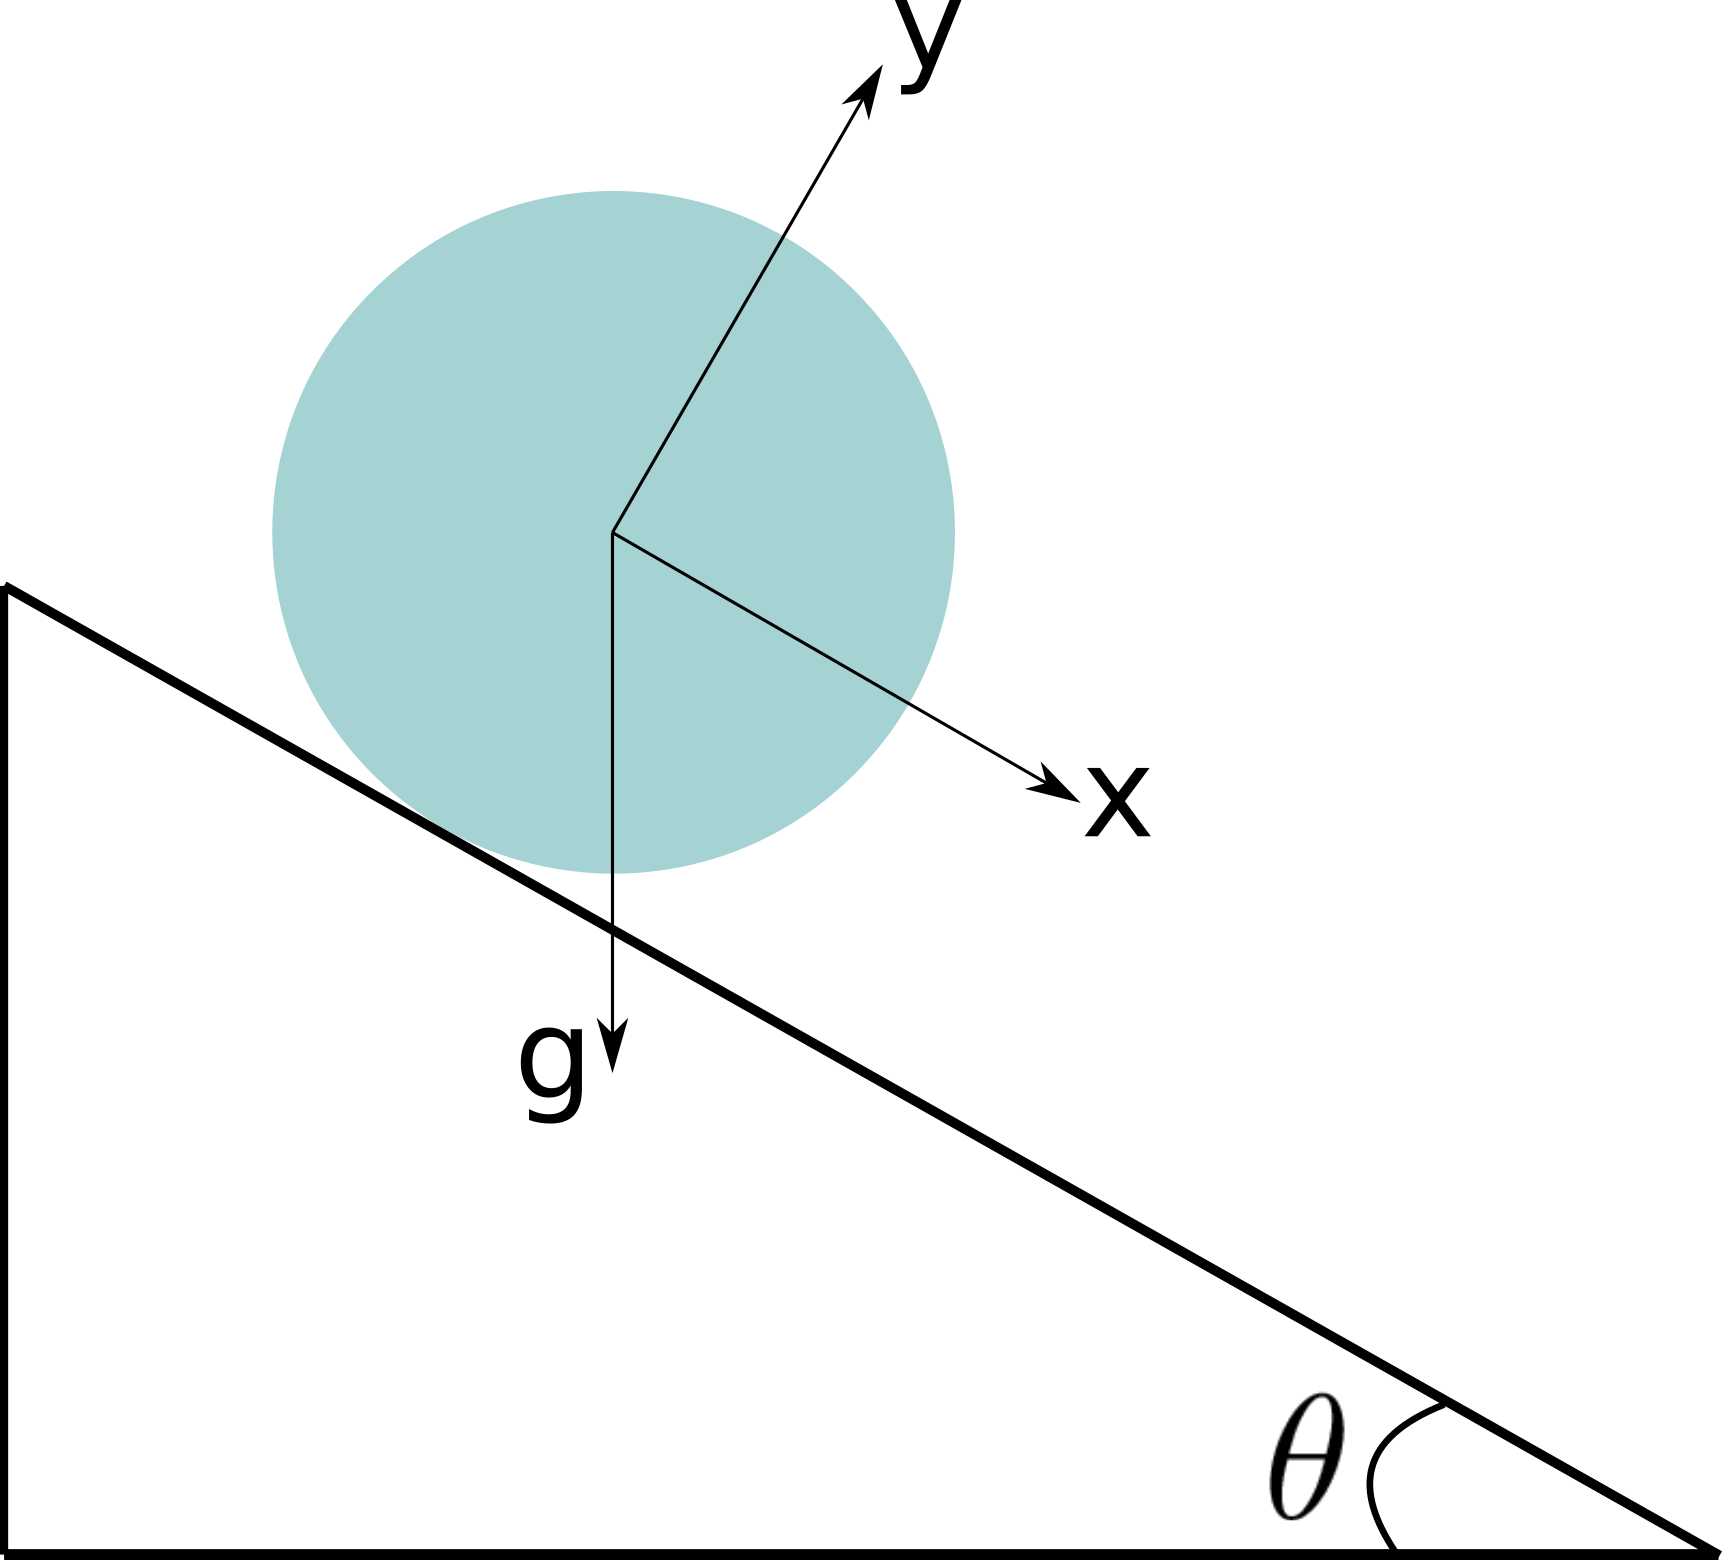
\includegraphics[width=1.0\textwidth]{images/de_2021_cylinder_rolling_on_an_inclined_plane/schematic_1}
    \subcaption{}\label{fig:circular-body:schematic-1}
  \end{subfigure}
  \begin{subfigure}{0.48\textwidth}
    \centering
    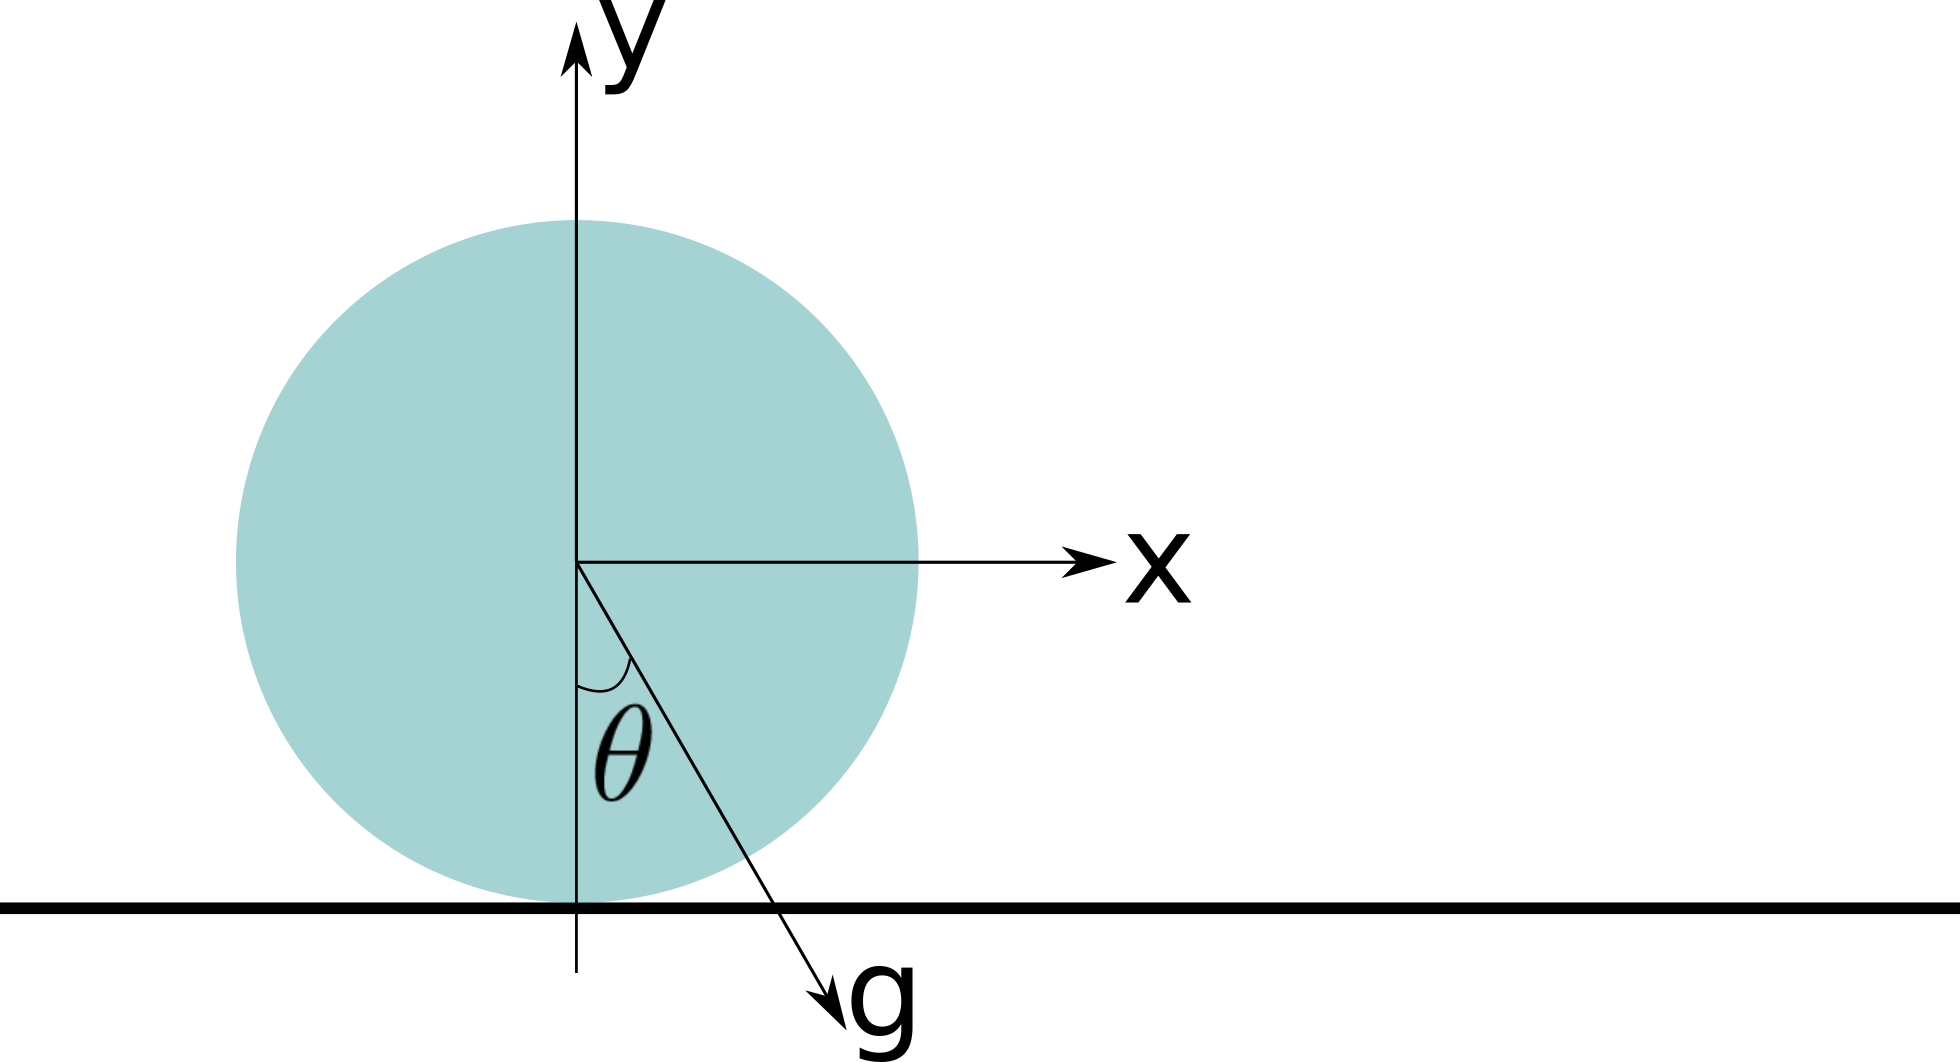
\includegraphics[width=1.0\textwidth]{images/de_2021_cylinder_rolling_on_an_inclined_plane/schematic_2}
    \subcaption{}\label{fig:circular-body:schematic-2}
  \end{subfigure}
  \caption{Curved interface}
\label{fig:circular-body-schematic}
\end{figure}
\begin{table}[!ht]
  \centering
  \begin{tabular}[!ht]{ll}
    \toprule
    Quantity & Values\\
    \midrule
    $\rho$, density & $2700$ kg\,m\textsuperscript{-3} \\
    $\mu$, friction coefficient & $0.3$ \& $0.6$ \\
    Time of simulation & $0.6$ s \\
    Resolution, $\delta x$ & $0.0025$ m\\
    Smoothing length factor, $h/\Delta x$ & 1\\
    gravity $[g_x, g_y, g_z]$ & $[g\,\sin(\theta), g\,\cos(\theta), 0.0]$\\
    $k_r$, Repulsive stiffness coefficient & $1e7$ \\
    $k_f$, Repulsive stiffness coefficient & $1e5$ \\
    $\alpha_{damp}$ & FIXME\\
    \bottomrule
  \end{tabular}
  \caption{Material properties and numerical parameters used for the rolling
    of cylinder on an inclined surface.}%
  \label{tab:circular-body-rolling-params}
\end{table}

\Cref{fig:cylinder-xcom-vs-time-fric-0-3} and
\cref{fig:cylinder-xcom-vs-time-fric-0-3} depicts the variation of center of
mass of the cylinder with time for a friction coefficients of $0.3$ and $0.6$.
From both the figures we can see that the center of mass predicted by the
current solver is at an excellent agreement with the exact solution. Further
\todo{put the right figure} \cref{fig:cylinder-xcom-vs-time-fric-0-3} shows
the snapshots of the cylinder at different time stamps, from which we can see
that the current scheme is stable.

\begin{figure}[!htpb]
  \centering
  \includegraphics[width=0.4\textwidth]{figures/de_2021_cylinder_rolling_on_an_inclined_plane_2d/fric_coeff_0_3/xcom_vs_time}
  \caption{x com vs time of a cylinder with a friction coefficient of $0.3$.}
\label{fig:cylinder-xcom-vs-time-fric-0-3}
\end{figure}

\begin{figure}[!htpb]
  \centering
  \includegraphics[width=0.4\textwidth]{figures/de_2021_cylinder_rolling_on_an_inclined_plane_2d/fric_coeff_0_6/xcom_vs_time}
  \caption{x com vs time of a cylinder with a friction coefficient of $0.6$.}
\label{fig:cylinder-xcom-vs-time-fric-0-6}
\end{figure}


\FloatBarrier%
\subsection{Three bodies colliding}
\label{sec:three-bodies-colliding}


\begin{figure}[!htpb]
  \centering
  % \includegraphics[width=0.4\textwidth]{figures/mohseni_2021_free_sliding_on_a_slope_3d/velocity_vs_time}
  \caption{Schematic of the three rigid body colliding}
\label{fig:schematic-three-rigid-bodies-colliding}
\end{figure}

\begin{figure}[!htpb]
  \centering
  \begin{subfigure}{0.48\textwidth}
    \centering
    \includegraphics[width=1.0\textwidth]{figures/amaro_2019_collision_between_three_rigid_cubes/Mohseni_Vyas/time0}
  \end{subfigure}
  %
  \begin{subfigure}{0.48\textwidth}
    \centering
    \includegraphics[width=1.0\textwidth]{figures/amaro_2019_collision_between_three_rigid_cubes/Mohseni_Vyas/time1}
  \end{subfigure}

  \begin{subfigure}{0.48\textwidth}
    \centering
    \includegraphics[width=1.0\textwidth]{figures/amaro_2019_collision_between_three_rigid_cubes/Mohseni_Vyas/time2}
  \end{subfigure}
  %
  \begin{subfigure}{0.48\textwidth}
    \centering
    \includegraphics[width=1.0\textwidth]{figures/amaro_2019_collision_between_three_rigid_cubes/Mohseni_Vyas/time3}
  \end{subfigure}
\caption{A dummy figure (To be fixed)}
\label{fig:snapshots-three-cubes-colliding}
\end{figure}
%


\FloatBarrier%
\subsection{Stack of cylinders}
\label{sec:stack-of-cylinders}

This test case is used to validate the current solid-solid contact force
model. A stack of cylinders initially at rest are allowed to settle under
gravity in a tank. This is simulated by Zhang (2011), where DEM is used. The
numerical parameters of the current test case are listed in
\Cref{tab:stack-of-cylinders}. The dimensions of the cylinder as well as the
tank are shown in figure (Ref the schematic figure).

\begin{table}[!ht]
  \centering
  \begin{tabular}[!ht]{ll}
    \toprule
    Quantity & Values\\
    \midrule
    $L$, length of the domain & 1 m \\
    Time of simulation & 2.5 s \\
    $c_s$ & 10 m/s \\
    $\rho_0$, reference density & 1 kg/m\textsuperscript{3} \\
    Reynolds number & 200 \& 1000 \\
    Resolution, $L/\Delta x_{\max} : L/\Delta x_{\min}$ & $[100:200]$ \& $[150:300]$\\
    Smoothing length factor, $h/\Delta x$ & 1.0\\
    \bottomrule
  \end{tabular}
  \caption{Parameters used for the Taylor-Green vortex problem.}%
  \label{tab:stack-of-cylinders}
\end{table}

\Cref{fig:snapshots-stack-of-cylinders} presents a set of snapshots
corresponding to the simulation of a stack of cylinders collapsing under
gravity using CTVF-DEM in comparison with the corresponding experimental
photos by Zhang. From the presented figure, the reproduced cylinder's
positions appear to be consistent with those observed in the experiment. From
\Cref{fig:snapshots-stack-of-cylinders}, the current solver has presented
proper level of stability.



\begin{figure}[!htpb]
  \centering
  \begin{subfigure}{0.48\textwidth}
    \centering
    \includegraphics[width=1.0\textwidth]{figures/stack_of_cylinders_2d/Mohseni_Vyas/time0}
  \end{subfigure}
  %
  \begin{subfigure}{0.48\textwidth}
    \centering
    \includegraphics[width=0.75\textwidth]{images/stack_of_cylinders_experimental_images/time0}
  \end{subfigure}

  \begin{subfigure}{0.48\textwidth}
    \centering
    \includegraphics[width=1.0\textwidth]{figures/stack_of_cylinders_2d/Mohseni_Vyas/time1}
  \end{subfigure}
  %
  \begin{subfigure}{0.48\textwidth}
    \centering
    \includegraphics[width=0.75\textwidth]{images/stack_of_cylinders_experimental_images/time1}
  \end{subfigure}

  \begin{subfigure}{0.48\textwidth}
    \centering
    \includegraphics[width=1.0\textwidth]{figures/stack_of_cylinders_2d/Mohseni_Vyas/time2}
  \end{subfigure}
  %
  \begin{subfigure}{0.48\textwidth}
    \centering
    \includegraphics[width=0.75\textwidth]{images/stack_of_cylinders_experimental_images/time2}
  \end{subfigure}

  \begin{subfigure}{0.48\textwidth}
    \centering
    \includegraphics[width=1.0\textwidth]{figures/stack_of_cylinders_2d/Mohseni_Vyas/time3}
  \end{subfigure}
  %
  \begin{subfigure}{0.48\textwidth}
    \centering
    \includegraphics[width=0.75\textwidth]{images/stack_of_cylinders_experimental_images/time3}
  \end{subfigure}
\caption{A dummy figure (To be fixed)}
\label{fig:snapshots-stack-of-cylinders}
\end{figure}
%



\Cref{fig:x-com-stack-of-cylinders,fig:y-com-stack-of-cylinders} presents the
time histories of the x and y components of the center of mass of the
cylinders respectively as well as those from numerical simulations by
SPH-DCDEM as well as MPS-DEM with respect to those from the experiment Zhang.
From the presented figure, the effective center of mass of the cylinders is in
good agreement with the experiment.

\begin{figure}[!htpb]
  \centering
  \includegraphics[width=0.4\textwidth]{figures/stack_of_cylinders_2d/Mohseni_Vyas/xcom}
  \caption{A dummy figure (To be fixed)}
\label{fig:x-com-stack-of-cylinders}
\end{figure}
\begin{figure}[!htpb]
  \centering
  \includegraphics[width=0.4\textwidth]{figures/stack_of_cylinders_2d/Mohseni_Vyas/ycom}
  \caption{A dummy figure (To be fixed)}
\label{fig:y-com-stack-of-cylinders}
\end{figure}


\FloatBarrier%
\subsection{Falling solid in water}
\label{sec:falling-solid-in-water}

In this section, the rigid fluid coupling part of the current solver is
evaluated by simulation of a rigid cube falling in an hydrostatic tank (cite
experimental paper). The CTVF-DEM solver is employed to simulate water entry
of a rigid cube, which is studied experimentally by (cite the paper). The
numerical parameters of the current test case are listed in
\Cref{tab:stack-of-cylinders}. The dimensions of the schematic are shown in
figure.

\begin{table}[!ht]
  \centering
  \begin{tabular}[!ht]{ll}
    \toprule
    Quantity & Values\\
    \midrule
    $L$, length of the domain & 1 m \\
    Time of simulation & 2.5 s \\
    $c_s$ & 10 m/s \\
    $\rho_0$, reference density & 1 kg/m\textsuperscript{3} \\
    Reynolds number & 200 \& 1000 \\
    Resolution, $L/\Delta x_{\max} : L/\Delta x_{\min}$ & $[100:200]$ \& $[150:300]$\\
    Smoothing length factor, $h/\Delta x$ & 1.0\\
    \bottomrule
  \end{tabular}
  \caption{Parameters used for the Taylor-Green vortex problem.}%
  \label{tab:stack-of-cylinders}
\end{table}

A rigid cube of a side length of 30 mm enters the water initially at
hydrostatic state with a velocity of 30 $m/s$ in z-direction.
\Cref{fig:snapshots-falling-solid-in-water} presents a snapshots of the rigid
cube falling in an hydrostatic tank with the current solver as well as
WCSPH-DEM solver as well as the experimental result. From the presented figure
\Cref{fig:snapshots-falling-solid-in-water}, we can see that the pressure
distribution is smooth and the simulation is stable. A zoomed in view near the
rigid cube is presented in \cref{fig:snapshots-falling-solid-in-water-zoomed}
when simulated with WCSPH-DEM and CTVF-DEM. From
\cref{fig:snapshots-falling-solid-in-water-zoomed} we can see that the fluid
particle distribution around the body with CTVF scheme is uniform when
compared with WCSPH, thanks to the implemented transport velocity formulation.

\begin{figure}[!htpb]
  \centering
  \begin{subfigure}{0.48\textwidth}
    \centering
    \includegraphics[width=1.0\textwidth]{figures/qiu_2017_falling_solid_in_water_2d/dx_0_002/time0}
  \end{subfigure}
  %
  \begin{subfigure}{0.48\textwidth}
    \centering
    \includegraphics[width=1.0\textwidth]{figures/qiu_2017_falling_solid_in_water_2d/dx_0_002/time1}
  \end{subfigure}

  \begin{subfigure}{0.48\textwidth}
    \centering
    \includegraphics[width=1.0\textwidth]{figures/qiu_2017_falling_solid_in_water_2d/dx_0_002/time2}
  \end{subfigure}
  %
  \begin{subfigure}{0.48\textwidth}
    \centering
    \includegraphics[width=1.0\textwidth]{figures/qiu_2017_falling_solid_in_water_2d/dx_0_002/time3}
  \end{subfigure}
\caption{A dummy figure (To be fixed)}
\label{fig:snapshots-falling-solid-in-water}
\end{figure}

\begin{figure}[!htpb]
  \centering
  \begin{subfigure}{0.48\textwidth}
    \centering
    \includegraphics[width=1.0\textwidth]{figures/qiu_2017_falling_solid_in_water_2d/dx_0_002/time0}
  \end{subfigure}
  %
  \begin{subfigure}{0.48\textwidth}
    \centering
    \includegraphics[width=1.0\textwidth]{figures/qiu_2017_falling_solid_in_water_2d/dx_0_002/time1}
  \end{subfigure}

  \begin{subfigure}{0.48\textwidth}
    \centering
    \includegraphics[width=1.0\textwidth]{figures/qiu_2017_falling_solid_in_water_2d/dx_0_002/time2}
  \end{subfigure}
  %
  \begin{subfigure}{0.48\textwidth}
    \centering
    \includegraphics[width=1.0\textwidth]{figures/qiu_2017_falling_solid_in_water_2d/dx_0_002/time3}
  \end{subfigure}
  \caption{Zoomed in snapshots of rigid body inside water.}
\label{fig:snapshots-falling-solid-in-water-zoomed}
\end{figure}

\Cref{fig:disp-falling-solid-in-water} presents the time history of the
displacement of the rigid cube with time in comparison with the experimental
result by (cite experimental paper). From the presented figure, the CTVF-DEM
model has reproduced the displacement of the rigid cube with acceptable levels
of stability as well as accuracy.
\begin{figure}[!htpb]
  \centering
  \includegraphics[width=0.4\textwidth]{figures/qiu_2017_falling_solid_in_water_2d/y_cm_vs_time}
  \caption{Center of mass of rigid body vs time compared with experiment}
\label{fig:disp-falling-solid-in-water}
\end{figure}


\FloatBarrier%
\subsection{3D dam breaking flow hitting cubes}

\cite{amaro2019improvement}

In the current case we simulate a 3d dam breaking flow hitting different
configuration of rigid cubes. This is experimentally studied by SPH DCDEM,
where the author used Direct Linear Transform (DLT) to track the cubes as they
move after the impact. A total three rigid body configurations are studied, a
single cube, three cubes and a pyramid configuration, respectively. It is
numerically studied by SPH-DCDEM, MPS-DEM, and (cite some other papers). The
side length of each cube is $3.5$ mm and the material properties are listed in
\cref{tab:material-properties-3d-dam-breaking-flow-hitting-cubes} and the
numerical parameters are given in
\cref{tab:material-properties-3d-dam-breaking-flow-hitting-cubes}. In all the
three cases the fluid is initially allowed to flow by opening a gate which
lifts at a velocity of 3.5 m\,s\textsuperscript{-1}

\begin{table}[!ht]
  \centering
  \begin{tabular}[!ht]{ll}
    \toprule
    Quantity & Values\\
    \midrule
    $L$, length of the domain & 1 m \\
    $\rho_0$, reference density & 1 kg/m\textsuperscript{3} \\
    Reynolds number & 200 \& 1000 \\
    Resolution, $L/\Delta x_{\max} : L/\Delta x_{\min}$ & $[100:200]$ \& $[150:300]$\\
    \bottomrule
  \end{tabular}
  \caption{Parameters used for the Taylor-Green vortex problem.}%
  \label{tab:material-properties-3d-dam-breaking-flow-hitting-cubes}
\end{table}

\begin{table}[!ht]
  \centering
  \begin{tabular}[!ht]{ll}
    \toprule
    Quantity & Values\\
    \midrule
    $L$, length of the domain & 1 m \\
    $\rho_0$, reference density & 1 kg/m\textsuperscript{3} \\
    Reynolds number & 200 \& 1000 \\
    Resolution, $L/\Delta x_{\max} : L/\Delta x_{\min}$ & $[100:200]$ \& $[150:300]$\\
    \bottomrule
  \end{tabular}
  \caption{Parameters used for the Taylor-Green vortex problem.}%
  \label{tab:numerical-properties-3d-dam-breaking-flow-hitting-cubes}
\end{table}

\Cref{fig:snapshots-single-cube-3d-dam-breaking-flow} shows the snapshots of
the rigid cube moving downstream of the tank when interacting with the fluid
flow against the experimental result (cite SPH DCDEM). From
\Cref{fig:snapshots-single-cube-3d-dam-breaking-flow} we can see that the
rigid cube matches well with the experimental result. Further, we compare the
positions of the rigid cube with time in
\Cref{fig:x-position-single-cube-3d-dam-breaking-flow}, against the
experimental results, SPH-DCDEM, MPS-DEM results. It can be seen from figure
\Cref{fig:x-position-single-cube-3d-dam-breaking-flow} that the current solver
is able to provide good accuracy in producing the correct displacement of the
cube and agrees well with the experimental as well as the other numerical
techniques.
\begin{figure}[!htpb]
  \centering
  \includegraphics[width=0.4\textwidth]{figures/mohseni_2021_free_sliding_on_a_slope_3d/velocity_vs_time}
  \caption{Snapshots of a single cube under a 3d dam breaking flow}
\label{fig:snapshots-single-cube-3d-dam-breaking-flow}
\end{figure}
\begin{figure}[!htpb]
  \centering
  \includegraphics[width=0.4\textwidth]{figures/mohseni_2021_free_sliding_on_a_slope_3d/velocity_vs_time}
  \caption{x position of the cube with time for single cube.}
\label{fig:x-position-single-cube-3d-dam-breaking-flow}
\end{figure}

The initial configuration of the dam breaking flow over three cubes is shown
in figure \Cref{fig:snapshots-three-cubes-3d-dam-breaking-flow}.
\Cref{fig:snapshots-three-cubes-3d-dam-breaking-flow} shows the snapshots of
the rigid cubes at different time instants from the start of fluid hit with
the color of the fluid particles representing pressure. From the
\Cref{fig:snapshots-three-cubes-3d-dam-breaking-flow} we can see that the
simulated rigid bodies match well with the experimental observations. We also
compare the x component of the effective center of mass of the three cubes
with time in \Cref{fig:x-position-three-cubes-3d-dam-breaking-flow}, against
the experimental results, SPH-DCDEM, MPS-DEM results. From figure
\Cref{fig:x-position-three-cubes-3d-dam-breaking-flow}, we can see that the
current solve is agrees well with the experimental as well as with the other
numerical method results.
\begin{itemize}
\item Mention at what time does the fluid hits the rigid cubes.
\end{itemize}
\begin{figure}[!htpb]
  \centering
  \includegraphics[width=0.4\textwidth]{figures/mohseni_2021_free_sliding_on_a_slope_3d/velocity_vs_time}
  \caption{Snapshots of a three cubes under a 3d dam breaking flow}
\label{fig:snapshots-three-cubes-3d-dam-breaking-flow}
\end{figure}
\begin{figure}[!htpb]
  \centering
  \includegraphics[width=0.4\textwidth]{figures/mohseni_2021_free_sliding_on_a_slope_3d/velocity_vs_time}
  \caption{x position of the cubes with time for three cube.}
\label{fig:x-position-three-cubes-3d-dam-breaking-flow}
\end{figure}


The placement of the cubes in the pyramid configuration including dimensions,
distance from the left wall and other dimension related information can be
seen in figure \Cref{fig:snapshots-three-cubes-3d-dam-breaking-flow}.
\Cref{fig:snapshots-three-cubes-3d-dam-breaking-flow} shows the snapshots of
the rigid cubes at different time instants and the color coding of the fluid
particles represents pressure. From
\Cref{fig:snapshots-three-cubes-3d-dam-breaking-flow}, it can be seen that the
rigid body positions are in match with the experimental observations. Which is
further validated by doing a quantitative comparison of the x component of
effective center of mass of the six cubes in time against the experimental
results, SPH-DCDEM, MPS-DEM results in
\Cref{fig:x-position-three-cubes-3d-dam-breaking-flow}. From these figures, we
can see that the current solver is in good agreement with the other numerical
and experimental results.
\begin{figure}[!htpb]
  \centering
  \includegraphics[width=0.4\textwidth]{figures/mohseni_2021_free_sliding_on_a_slope_3d/velocity_vs_time}
  \caption{Snapshots of six cubes under a 3d dam breaking flow}
\label{fig:snapshots-six-cubes-3d-dam-breaking-flow}
\end{figure}
\begin{figure}[!htpb]
  \centering
  \includegraphics[width=0.4\textwidth]{figures/mohseni_2021_free_sliding_on_a_slope_3d/velocity_vs_time}
  \caption{x position of the six with time for three cube.}
\label{fig:x-position-six-cube-3d-dam-breaking-flow}
\end{figure}

% \subsection{Dam break with body transport}
% \label{sec:dam-break-with-body-transport}

% \citet{wang2019numerical}

% \subsection{Dam break with multiple bodies transport}
% \label{sec:dam-break-with-multiple-bodies-transport}
% \citet{wang2019numerical}


% \subsection{Cylinders in water collapsed under gravity}
% \label{sec:cylinders-collapse-in-water}
% \citet{chen2019coupled}


\section{Conclusions}
\label{sec:conclusions}

\section*{References}
\bibliographystyle{model6-num-names}
\bibliography{references}



\end{document}

%%% Local Variables:
%%% mode: latex
%%% TeX-master: "paper"
%%% fill-column: 78
%%% End:
